\documentclass[12pt,letterpaper]{article}
\usepackage[utf8]{inputenc}
\usepackage[spanish]{babel}
\usepackage{graphicx}
\usepackage[left=2cm,right=2cm,top=2cm,bottom=2cm]{geometry}
\usepackage{graphicx} % figuras
% \usepackage{subfigure} % subfiguras
\usepackage{float} % para usar [H]
\usepackage{amsmath}
%\usepackage{txfonts}
\usepackage{stackrel} 
\usepackage{multirow}
\usepackage{enumerate} % enumerados
\renewcommand{\labelitemi}{$-$}
\renewcommand{\labelitemii}{$\cdot$}
% \author{}
% \title{Caratula}
\begin{document}

% Fancy Header and Footer
% \usepackage{fancyhdr}
% \pagestyle{fancy}
% \cfoot{}
% \rfoot{\thepage}
%

% \usepackage[hidelinks]{hyperref} % CREA HYPERVINCULOS EN INDICE

% \author{}
\title{Caratula}

\begin{titlepage}
\begin{center}
\large{UNIVERSIDAD PRIVADA-DE-TACNA}\\
\vspace*{-0.025in}
\begin{figure}[htb]
\begin{center}

\includegraphics[width=8cm]{./Imagenes/logo}
\end{center}
\end{figure}
\vspace*{0.15in}
INGENIERIA DE SISTEMAS  \\
\vspace*{0.5in}
\begin{large}
TITULO:\\
\end{large}
\vspace*{0.1in}
\begin{Large}
\textbf{INFORME DE LABORATORIO Nº 04} \\
\end{Large}
\vspace*{0.3in}
\begin{Large}
\textbf{CURSO:} \\
\end{Large}
\vspace*{0.1in}
\begin{large}
BASE DE DATOS II\\
\end{large}
\vspace*{0.3in}
\begin{Large}
\textbf{DOCENTE(ING):} \\
\end{Large}
\vspace*{0.1in}
\begin{large}
 Patrick Cuadros Quiroga\\
\end{large}
\vspace*{0.2in}
\vspace*{0.1in}
\begin{large}
Integrantes: \\
\begin{flushleft}
Acosta Ortiz, Orlando Antonio                  \hfill	(2015052775) \\
Ramirez Ticona, Orestes                           \hfill  (2015053236) \\
Zegarra Reyes, Roberto  		            \hfill 	(2010036175) \\
Catari Cabrera, Yofer Nain 		\hfill 	(2017059289) \\
Mamani Maquera, Jorge Luis                   \hfill 	(2016055236) \\
Rivas Rios, Marko Antonio                       \hfill 	(2016054461) \\
\end{flushleft}
\end{large}
\end{center}

\end{titlepage}


\tableofcontents % INDICE
\thispagestyle{empty} % INDICE SIN NUMERO
\newpage
\setcounter{page}{1} % REINICIAR CONTADOR DE PAGINAS DESPUES DEL INDICE

\section{INFORMACIÓN GENERAL} 

\begin{itemize}
\subsection{Objetivos:}

	 \item Aprender sobre como iniciar la Instalacion  de una Instancia de Microsoft SQL
\subsection{Requerimientos}

	
	\textbf{Conocimientos}\\
	 
	
    Para el desarrollo de esta práctica se requerirá de los siguientes        	  conocimientos básicos:
	\item Conocimientos básicos de administración de base de datos 	  			 Microsoft SQL Server.
	\item Conocimientos básicos de SQL.\\
	
	\textbf{Hardware}\\
	
	\item Virtualization activada en el BIOS..
	\item CPU SLAT-capable feature.
	\item Al menos 4GB de RAM.\\
	
	 \textbf{Software}\\
	
	Asimismo se necesita los siguientes aplicativos:
	\item Windows 10 64bit: Pro, Enterprise o Education (1607 Anniversary 			  Update, Build 14393 o Superior)
	\item Docker Desktop (Para lo cual se debe primero crear una cuenta en 			  Docker Hub - https://hub.docker.com/signup?next=%2Feditions	   			  %2Fcommunity%2Fdocker-ce-desktop-windows%3Fref%3Dlogin)
	\item Microsoft SQL Server Management Studio en su última versión



\end{itemize}
\section{MARCO TEORICO} 

Una instancia de Motor de base de datos es una copia del ejecutable de sqlservr.exe que se ejecuta como un servicio de sistema operativo. Cada instancia administra varias bases de datos del sistema y una o varias bases de datos de usuario. Cada equipo puede ejecutar varias instancias de Motor de base de datos. Las aplicaciones se conectan a la instancia para realizar el trabajo en una base de datos administrada por la instancia.

\textbf{Instancias}\\

Una instancia de Motor de base de datos funciona como un servicio que controla todas las solicitudes de aplicación para trabajar con datos de cualquiera de las bases de datos administradas por dicha instancia. Es el destino de las solicitudes de conexión (inicios de sesión) de aplicaciones. La conexión se ejecuta en una conexión de red si la aplicación y la instancia están en equipos independientes. Si la aplicación y la instancia están en el mismo equipo, la conexión de SQL Server se puede ejecutar como una conexión de red o una conexión en memoria. Cuando una conexión se ha completado, una aplicación envía instrucciones Transact-SQL a través de la conexión hasta la instancia. La instancia resuelve las instrucciones de Transact-SQL en operaciones con los datos y objetos de las bases de datos y, si se han concedido los permisos necesarios a las credenciales de inicio de sesión, realiza el trabajo. Los datos recuperados se devuelven a la aplicación, junto con cualesquiera mensajes como errores.
Puede ejecutar múltiples instancias de Motor de base de datos en un equipo. Una instancia puede ser la instancia predeterminada. La instancia predeterminada no tiene nombre. Si una solicitud de conexión especifica solo el nombre del equipo, se establece la conexión a la instancia predeterminada. Una instancia con nombre es una instancia en la que se especifica un nombre de instancia al instalar la instancia. Una solicitud de conexión debe especificar el nombre del equipo y el nombre de instancia para conectar a la instancia. No hay ningún requisito para instalar una instancia predeterminada; todas las instancias que se ejecutan en un equipo pueden ser instancias con nombre.


\section{PROCEDIMIENTO} 

\begin{itemize}
\subsection{Instalacion de Docker}
	
	\item Instalar Docker desde la siguiente direccion :
	https://docs.docker.com/docker-for-windows/install/
	\begin{figure}[htb]
	\begin{center}
	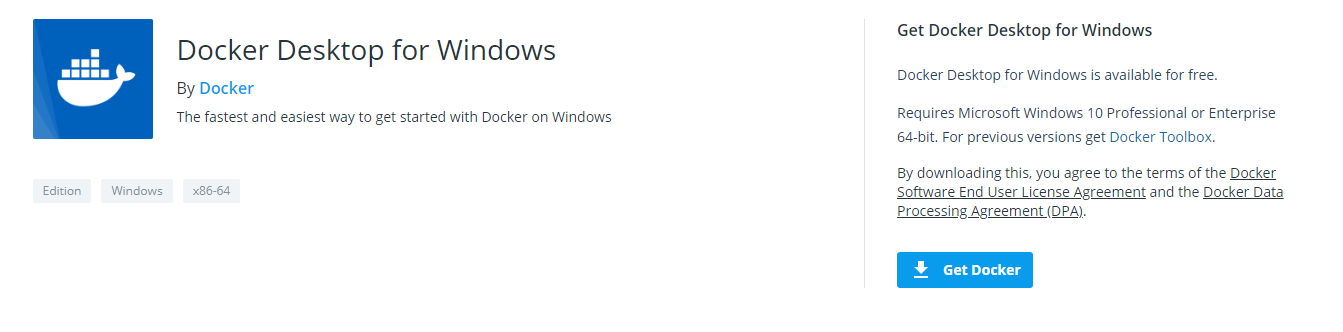
\includegraphics[width=18cm, height=8cm]{./Imagenes/docker}
	\end{center}
	\end{figure}\\
	
	\item Seguir el proceso de Instalacion :\\
	\begin{figure}[htb]
	\begin{center}
	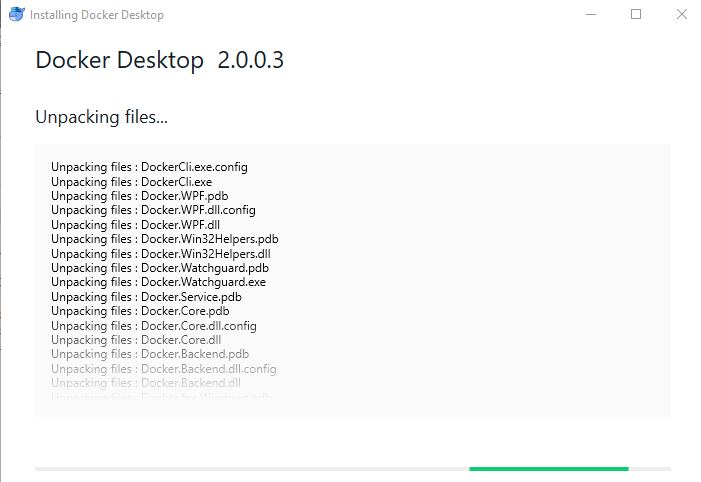
\includegraphics[width=18cm, height=8cm]{./Imagenes/dockerinst}
	\end{center}
	\end{figure}\\
	
	\item Reiniciar la PC :\\
	\begin{figure}[htb]
	\begin{center}
	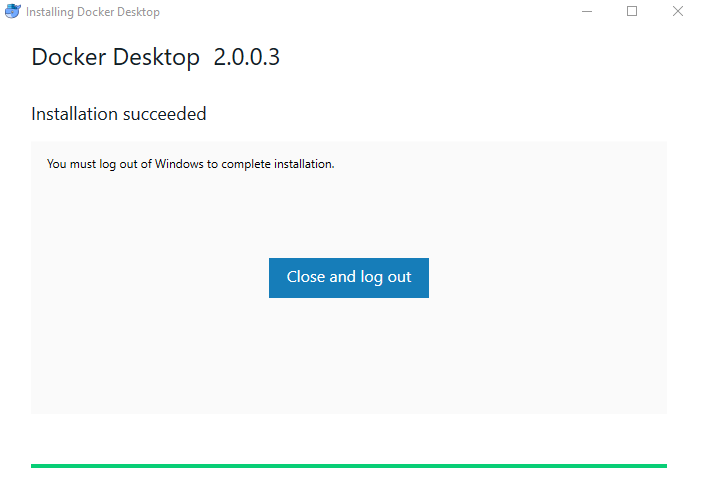
\includegraphics[width=18cm, height=8cm]{./Imagenes/dockerre}
	\end{center}
	\end{figure}
	
	\item Comprobar que docker ha sido instalado correctamente:\\	
	\begin{figure}[htb]
	\begin{center}
	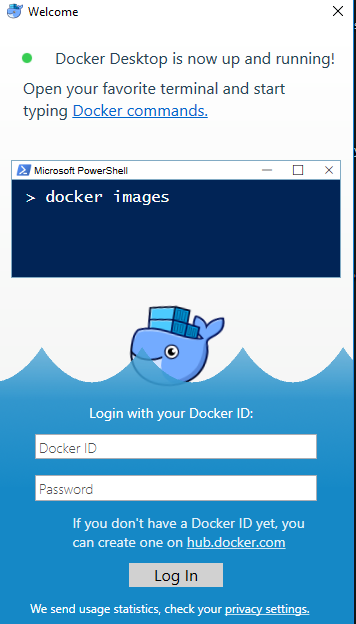
\includegraphics[width=7cm, height=8cm]{./Imagenes/dockerrun}
	\end{center}
	\end{figure}\\\\\\\\		
		
\subsection{Iniciando en Docker}
	
	\item Logearse con su cuenta y contraseña Respectiva:\\
			
	\begin{figure}[htb]
	\begin{center}
	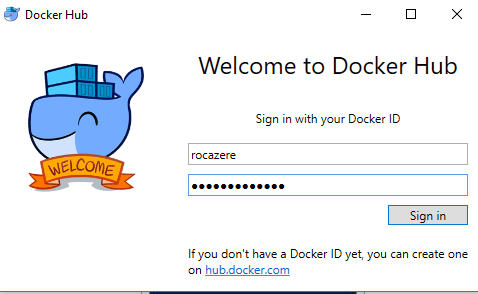
\includegraphics[width=8cm, height=6cm]{./Imagenes/dockerlogin}
	\end{center}
	\end{figure}
	
	\item Iniciar la consola PowerShell de Windows:\\
	
	\begin{figure}[htb]
	\begin{center}
	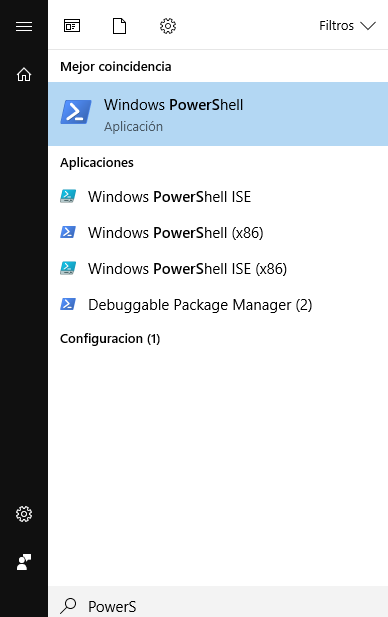
\includegraphics[width=8cm, height=10cm]{./Imagenes/powershell}
	\end{center}
	\end{figure}
	\clearpage
	
	\subsection{Creando un contenedor Miscrosoft SQL para Linux}
	
	\item Como primer comando usaremos:  "docker version" para ver la    version de docker que acabamos de instalar:\\
	
	
	\begin{figure}[htb]
	\begin{center}
	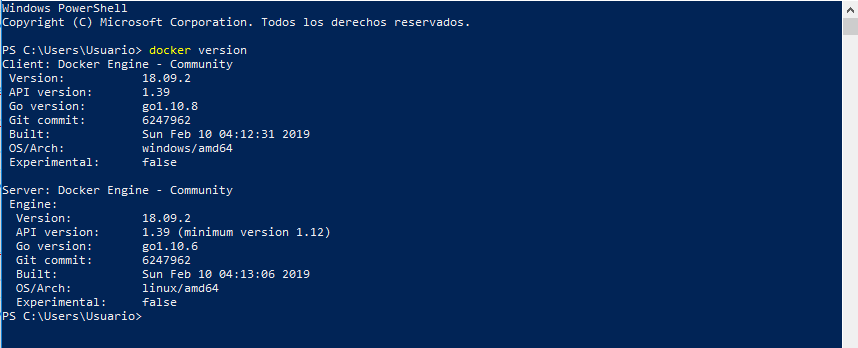
\includegraphics[width=16cm, height=8cm]{./Imagenes/dockerversion}
	\end{center}
	\end{figure}
	
	\item Ahora crearemos un contenedor con Microsoft SQL server para Linux, para esto usaremos primero el comando "docker search mssql":\\
	
	
	\begin{figure}[htb]
	\begin{center}
	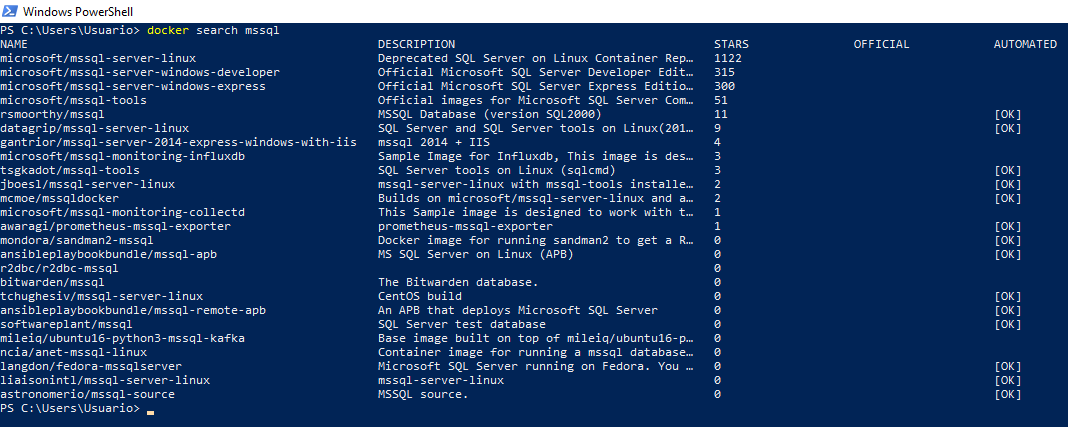
\includegraphics[width=16cm, height=8cm]{./Imagenes/dockersearch}
	\end{center}
	\end{figure}
	\clearpage
	
	\item Luego descargaremos la imagen del contenedor de Microsoft SQL en un servidor Linux con el siguiente comando "docker pull microsoft/mssql-server-linux":\\
	
	
	\begin{figure}[htb]
	\begin{center}
	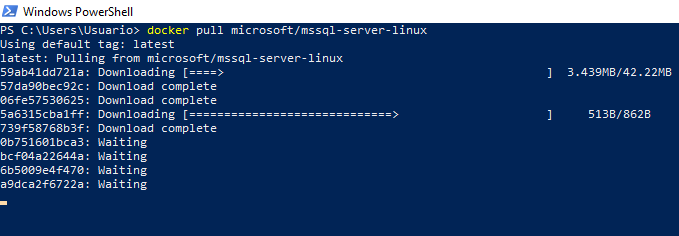
\includegraphics[width=16cm, height=8cm]{./Imagenes/dockerdownload}
	\end{center}
	\end{figure}
	
	\item esperar un determinado tiempo a que descargue todo:\\
	
	
	\begin{figure}[htb]
	\begin{center}
	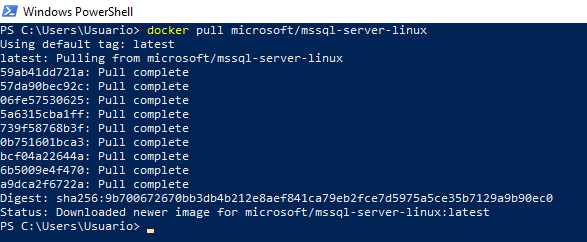
\includegraphics[width=16cm, height=8cm]{./Imagenes/dockerdownloaded}
	\end{center}
	\end{figure}
	\clearpage
	
	\item Para ver la imagen que acabamos de descargar, usaremos el siguiente comando: "docker images":\\
	
	
	\begin{figure}[htb]
	\begin{center}
	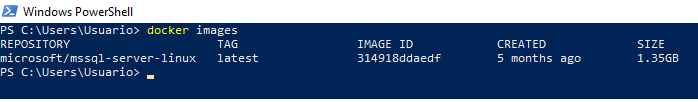
\includegraphics[width=16cm, height=3cm]{./Imagenes/dockerimages}
	\end{center}
	\end{figure}
	
	\item Ahora crearemos credenciales los cuales usaremos mas adelante para autenticar nuestra entrada a SQL server, usaremos el siguiente comando: 
	
	
	\begin{figure}[htb]
	\begin{center}
	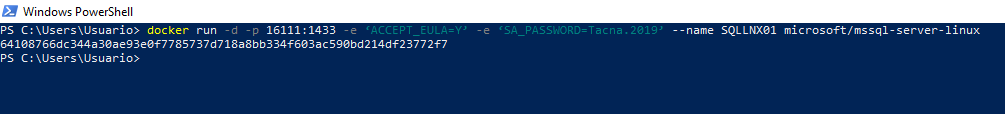
\includegraphics[width=16cm, height=3cm]{./Imagenes/dockercred}
	\end{center}
	\end{figure}
	
	\item Accedemos a dar los permisos para el firewall de Windows
	
	\begin{figure}[htb]
	\begin{center}
	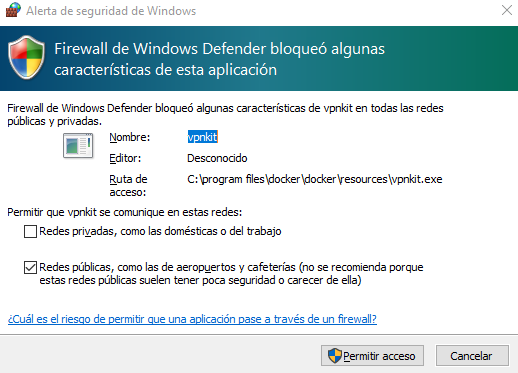
\includegraphics[width=10cm, height=9cm]{./Imagenes/firewall}
	\end{center}
	\end{figure}
	
	\item Verificamos la correcta ejecucion del contenedor con el comando "docker ps":\\
	
	\begin{figure}[htb]
	\begin{center}
	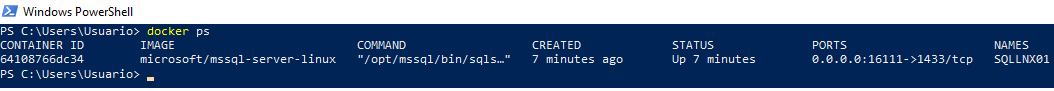
\includegraphics[width=16cm, height=2cm]{./Imagenes/dockerps}
	\end{center}
	\end{figure}
	
	\item Accedemos a Sql server con los siguientes credenciales:\\
	
	\begin{figure}[htb]
	\begin{center}
	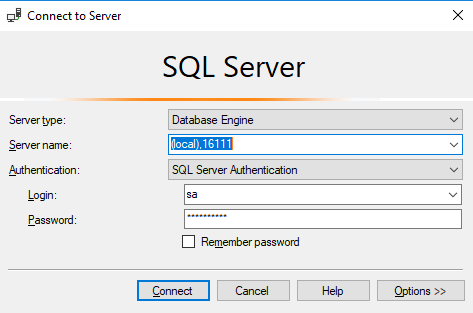
\includegraphics[width=10cm, height=9cm]{./Imagenes/sql}
	\end{center}
	\end{figure}
	
	\item En sql iniciairemos un nuevo query para hacer una consulta sobre la version:\\
	
	\begin{figure}[htb]
	\begin{center}
	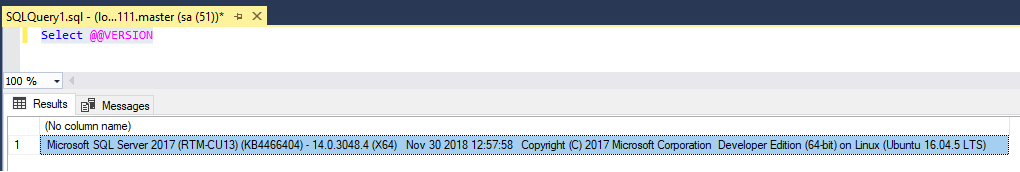
\includegraphics[width=18cm, height=4cm]{./Imagenes/sqlconsulta}
	\end{center}
	\end{figure}
	\clearpage
	\item Ahora cerraremos Sql server y procederemos a eliminar el contenedor creado con el siguiente comando: "docker rm -f SQLLNX01" y despues comprobaremos que este ha sido eliminado:\\
	
	\begin{figure}[htb]
	\begin{center}
	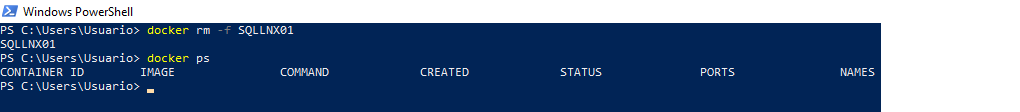
\includegraphics[width=21cm, height=4cm]{./Imagenes/dockerele}
	\end{center}
	\end{figure}
	\clearpage
	\subsection{Adicionando una Persistencia}
	
	\item Crearemos un nuevo contenedor, verificaremos que este ha sido creado correctamente y luego iniciaremos sesion con los respectivos credenciales:\\
	
	
	\begin{figure}[htb]
	\begin{center}
	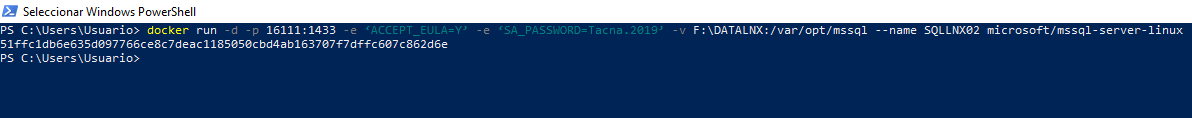
\includegraphics[width=16cm, height=4cm]{./Imagenes/daltan}
	\end{center}
	\end{figure}
	
	\begin{figure}[htb]
	\begin{center}
	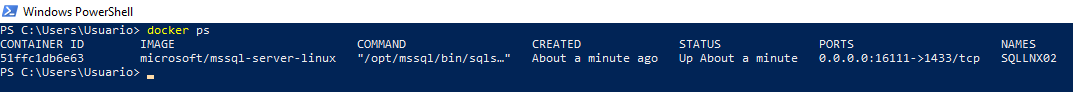
\includegraphics[width=16cm, height=4cm]{./Imagenes/dockerps2}
	\end{center}
	\end{figure}
	
	
	\begin{figure}[htb]
	\begin{center}
	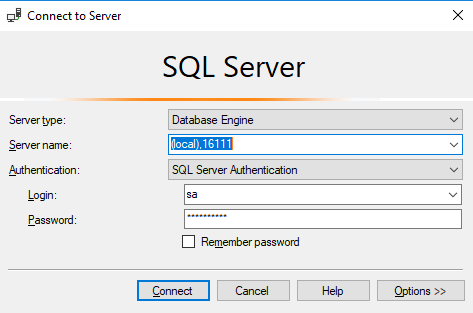
\includegraphics[width=9cm, height=7cm]{./Imagenes/sql}
	\end{center}
	\end{figure}
	\clearpage
	
	\item Ahora crearemos una base de datos con el siguiente Script:\\
	
	\begin{figure}[htb]
	\begin{center}
	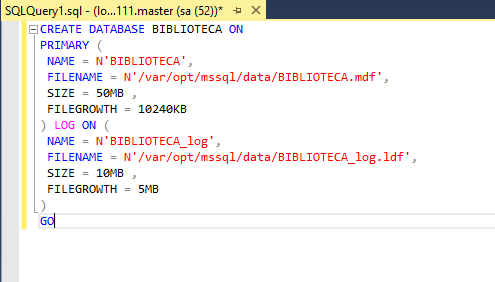
\includegraphics[width=19cm, height=8cm]{./Imagenes/script}
	\end{center}
	\end{figure}
	
	\item Verificaremos que la carpeta DATALNX contenga esta base de datos:\\
	
	\begin{figure}[htb]
	\begin{center}
	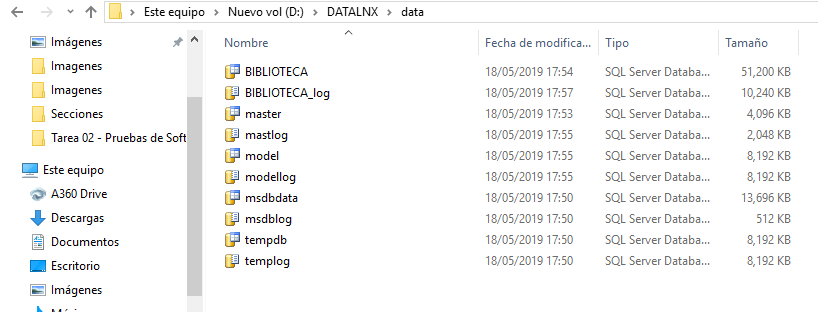
\includegraphics[width=19cm, height=8cm]{./Imagenes/datal}
	\end{center}
	\end{figure}
	
	\item Por ultimo eliminaremos este contenedor.\\
	\clearpage
	
	
	\subsection{Creando un contenedor con Microsoft SQL para Windows}
	
	\item En la parte inferior derecha encontraremos el icono de Docker el cual al hacerle click derecho, abrira un menu desplegable en el que seleccionaremos Switch to windows containers... y esperaremos a que docker se reinicie:\\
	
	\begin{figure}[htb]
	\begin{center}
	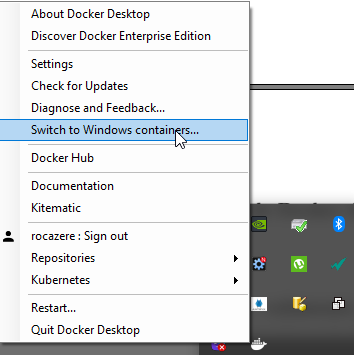
\includegraphics[width=17cm, height=7cm]{./Imagenes/winco}
	\end{center}
	\end{figure}
	
	\item Ahora en la ventana de PowerShell usaremos los siguientes comandos::\\
	
	
	\begin{figure}[htb]
	\begin{center}
	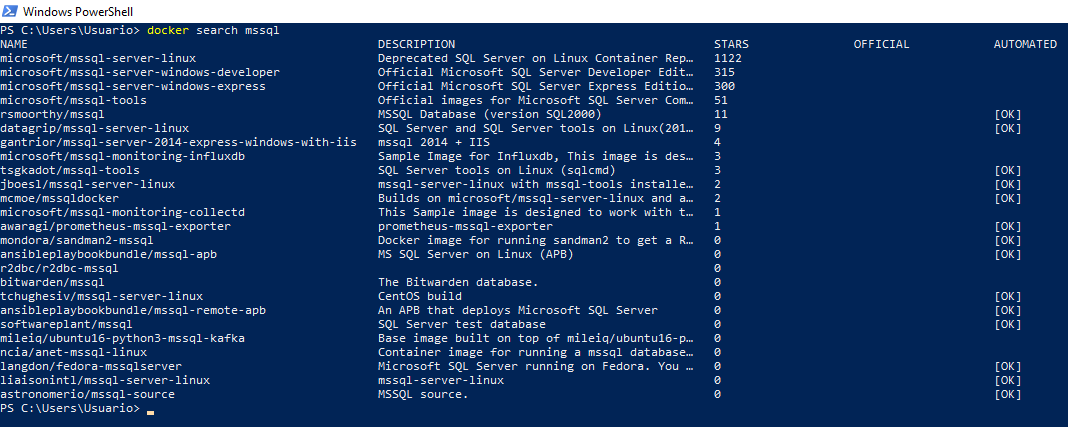
\includegraphics[width=17cm, height=7cm]{./Imagenes/dockersearch}
	\end{center}
	\end{figure}
	\clearpage
	\item Instalaremos el contenedor de Microsoft sql para un servidor Windows:\\
			
	\begin{figure}[htb]
	\begin{center}
	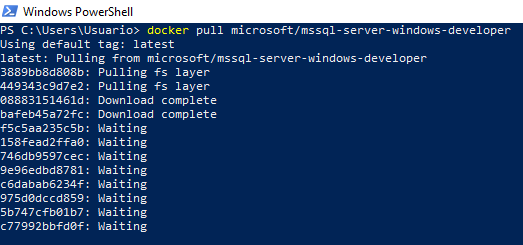
\includegraphics[width=17cm, height=7cm]{./Imagenes/windows}
	\end{center}
	\end{figure}
	
	\item Comprobaremos la correcta instalacion del contenedor con el comando "docker images":\\
	
	\begin{figure}[htb]
	\begin{center}
	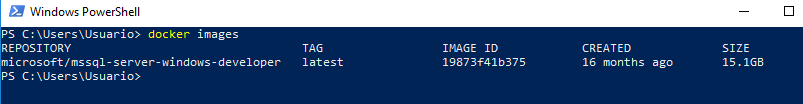
\includegraphics[width=15cm, height=5cm]{./Imagenes/windowsimages}
	\end{center}
	\end{figure}
	\clearpage
	
	\item Crearemos nuevos credenciales para este nuevo contenedor Sql para servidores windows:\\
	
	\begin{figure}[htb]
	\begin{center}
	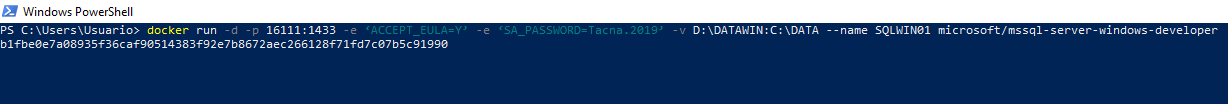
\includegraphics[width=20cm, height=3cm]{./Imagenes/credenciales}
	\end{center}
	\end{figure}
	
	\item Iniciaremos sesion en Sql con las credenciales que hemos creado:\\
	
	\begin{figure}[htb]
	\begin{center}
	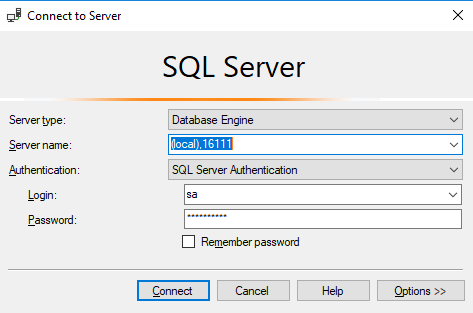
\includegraphics[width=10cm, height=9cm]{./Imagenes/sql}
	\end{center}
	\end{figure}
	\clearpage
	\item revisamos la version: 	
	
	\begin{figure}[htb]
	\begin{center}
	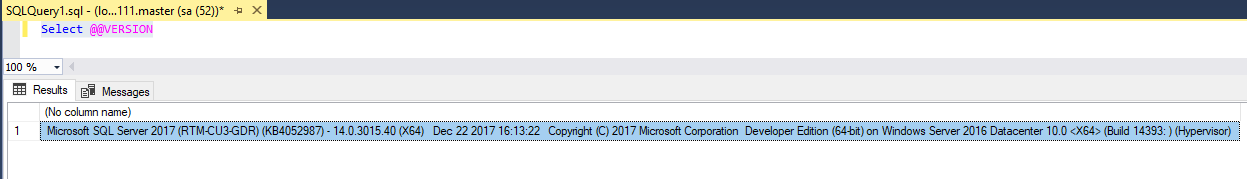
\includegraphics[width=18cm, height=4cm]{./Imagenes/sqlwindows}
	\end{center}
	\end{figure}
	
	\item Mediante el siguiente scrip generaremos una base de datos de prueba:\\
	
	\begin{figure}[htb]
	\begin{center}
	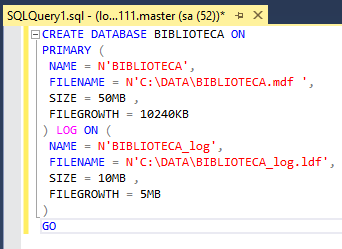
\includegraphics[width=10cm, height=8cm]{./Imagenes/scrip}
	\end{center}
	\end{figure}
	\clearpage
	\item Comprobaremos que la base de datos ha sido creada:\\
	
	\begin{figure}[htb]
	\begin{center}
	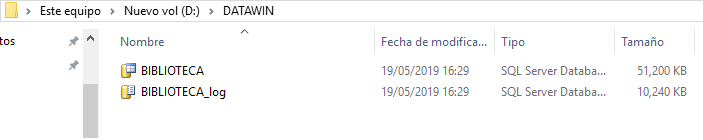
\includegraphics[width=16cm, height=4cm]{./Imagenes/datawin}
	\end{center}
	\end{figure}
	
	\item Finalmente procederemos con la eliminacion del conteneder y verificaremos que esta ha sido eliminada:\\
	
	\begin{figure}[htb]
	\begin{center}
	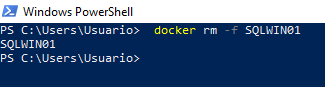
\includegraphics[width=10cm, height=5cm]{./Imagenes/dockerrm}
	\end{center}
	\end{figure}
	
	\begin{figure}[htb]
	\begin{center}
	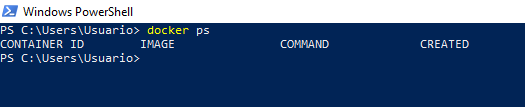
\includegraphics[width=12cm, height=3cm]{./Imagenes/dockerpsss}
	\end{center}
	\end{figure}
	\clearpage
	
	\subsection{Actividades Encargadas}
	
	\subsubsection{¿Con qué comando(s) exportaría la imagen de Docker de Microsoft SQL Server a otra PC o servidor?}
	
	\item uno de los comandos usados para exportar un contendor seria:
	
		\begin{figure}[htb]
	\begin{center}
	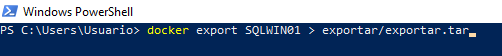
\includegraphics[width=12cm, height=3cm]{./Imagenes/tar}
	\end{center}
	\end{figure}
	
	Podemos observar que hemos guardar un archivo .tar en nuestra carpeta usuarios. Luego esto podra ser transportando ha otra maquina ya sea windows o linux.
		\begin{figure}[htb]
	\begin{center}
	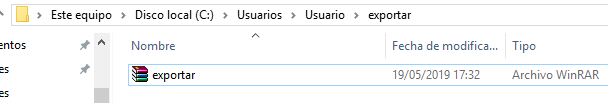
\includegraphics[width=12cm, height=3cm]{./Imagenes/tar2}
	\end{center}
	\end{figure}
	\clearpage
	
	
	
	\subsubsection{¿Con qué comando(s) podría generar dos volúmenes para un contenedor?}
	
	\item Los volumenes pueden ser gestionados con el siguiente comando:
	
	\begin{figure}[htb]
	\begin{center}
	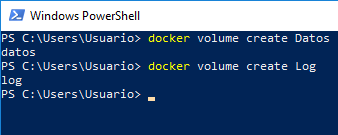
\includegraphics[width=12cm, height=3cm]{./Imagenes/volumenes}
	\end{center}
	\end{figure}
	
	\item Con el siguiente comando, podremos ver donde estos han sido creados:
	
	
	\begin{figure}[htb]
	\begin{center}
	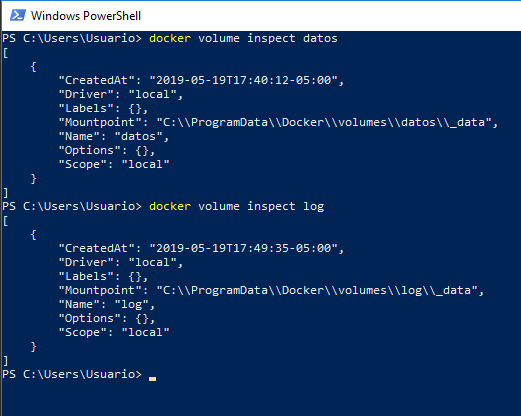
\includegraphics[width=10cm, height=9cm]{./Imagenes/volumenes2}
	\end{center}
	\end{figure}
	
	Ahora podremos usar estos volumens creado para crear nuestros archivos .mdf y .log en sus repectivos directorios.
	\clearpage
	
	
	
	\subsubsection{Genere un nuevo contenedor con las siguientes caracteristicas:}
	
	\item El Script es:
	
	\begin{figure}[htb]
	\begin{center}
	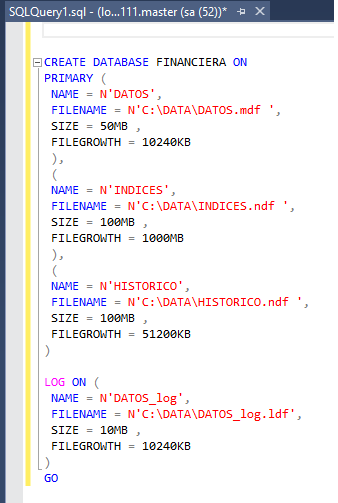
\includegraphics[width=10cm, height=9cm]{./Imagenes/scriptq}
	\end{center}
	\end{figure}
	
	\item Verificamos que haya sido creado correctamente:
	
	\begin{figure}[htb]
	\begin{center}
	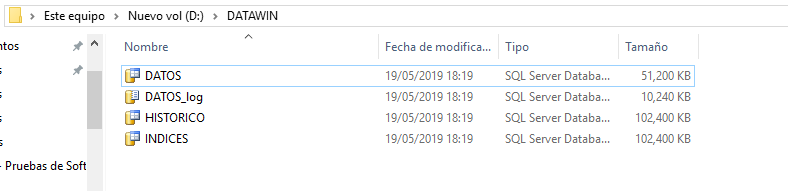
\includegraphics[width=10cm, height=6cm]{./Imagenes/scriptq2}
	\end{center}
	\end{figure}
	
	
	
	

\end{itemize}
\section{CUESTIONARIO} 
\begin{itemize}
\subsection{¿Con qué comando(s) exportaría la imagen de Docker de Microsoft SQL Server a otra PC o servidor?}
	\item linea
\subsection{¿Con qué comando(s) podría generar dos volúmenes para un contenedor para distribuir en un volumen el Archivo
de Datos (mdf) y en otro el Archivo Log (ldf)?}
	\item linea

\subsection{Genere un nuevo contenedor y cree la base de datos con las siguientes características}
\item ¿Cuál sería el script SQL que generaría esta base de datos?

\end{itemize}
\section{CONCLUSIONES} 

\begin{itemize}
	\item Aprendimos a crear contenedores para distintos tipos de Servidores, los contenedores nos ayudar a transpotar de manera facil y efiniciente las bases de datos entre diferentes tipos de Sistemas Operadores y servidores evitando asi la perdida y el desorden de datos.
	
	



\end{itemize}
\section{BIBLIOGRAFIA} 

\begin{itemize}
\item Aplicar y Desarrollar  Consultas con Pivot y Grouping Sets



\end{itemize}
\section{WEBGRAFIA} 

\begin{itemize}
\item https://dockertips.com/volumenes
\item https://cerebro-digital.com/panel/knowledgebase/64/ExportarorImportar-contenedor-de-Docker-via-archivo-TAR.html
\item  https://www.docker.com/
\item https://www.campusmvp.es/recursos/post/los-beneficios-de-utilizar-docker-y-contenedores-a-la-hora-de-programar.aspx

\end{itemize}
\end{document}
